Seguimos principalmente \cite{diestel2017}. Igualmente, algunas definiciones son tomadas de \cite{jafarian2013} y de \cite{gomez2025}.\\

Dado un conjunto $S$ y un número natural $k$, denotamos por $[S]^k$ a la colección de todos los subconjuntos de $S$ con exactamente $k$ elementos. Así por ejemplo, tomando $S=\left\lbrace 1,2,3,4,5 \right\rbrace$, tenemos que 
$$
[S]^3=\left\lbrace \left\lbrace 1,2,3\right\rbrace, \left\lbrace 1,2,4\right\rbrace, \left\lbrace 1,2,5\right\rbrace, \left\lbrace 1,3,4\right\rbrace, \left\lbrace 1,3,5\right\rbrace, \left\lbrace 1,4,5\right\rbrace, \left\lbrace 2,3,4\right\rbrace, \left\lbrace 2,3,5\right\rbrace, \left\lbrace 2,4,5\right\rbrace, \left\lbrace 3,4,5\right\rbrace\right\rbrace
$$
Los elementos de $[S]^k$ son llamados $k-subconjuntos$ de $S$. Con esto, damos la definición de grafo:
\begin{Def}
   Un \textbf{grafo} es una pareja $G=\left( V,A\right)$ de conjuntos tal que $A\subseteq [V]^2$. Los elementos de $V$ son llamados \textbf{vértices} y los elementos de $A$ son llamados \textbf{aristas}.
\end{Def}
De este modo, las aristas de un grafo son $2-subconjuntos$ de vértices. En general, dado un grafo $G$, denotaremos por $V(G)$ a su conjunto de vértices, y por $A(G)$ a su conjunto de aristas. Un grafo con conjunto de vértices $V$ también es llamado un \textit{grafo sobre V}. Para evitar ambiguedades de notación, asumimos también que $V(G)\cap A(G)=\phi$ para todo grafo $G$. Una arista $\left\lbrace u,v\right\rbrace$ de un grafo también puede ser representada mediante $uv$; en este caso nótese que $uv$ y $vu$ hacen referencia a la misma arista, pues $uv=\left\lbrace u,v\right\rbrace=\left\lbrace v, u\right\rbrace=vu$. Este tipo de grafos en los cuales el orden de los vértices en la representación de la arista no es tenido en cuenta también son llamados \textit{grafos no dirigidos}.
\begin{Ejm} \label{Ejm:cuatro_grafos}
   Los siguientes son ejemplos de grafos sobre $V=\left\lbrace v_1,v_2,v_3,v_4,v_5, v_6 \right\rbrace$:
   \begin{itemize}
      \item $G_1=(V,\left\lbrace v_1v_2,v_2v_3,v_3v_4,v_4v_5,v_5v_6, v_6v_1\right\rbrace)$
      \item $G_2=(V,\left\lbrace v_1v_2, v_2v_3, v_1v_3, v_3v_4, v_5v_6\right\rbrace)$
      \item $G_3=(V, \left\lbrace v_1v_2, v_1v_3, v_1v_4, v_1v_5, v_1v_6\right\rbrace)$
      \item $G_4=(V,\left\lbrace v_1v_4, v_2v_3, v_2v_5, v_2v_6, v_3v_4, v_3v_6, v_5v_6\right\rbrace)$
   \end{itemize}
   Un ejemplo de grafo sobre $V'=\left\lbrace v_1, v_2, v_3, \dots\right\rbrace$ es $G_5=(V',\left\lbrace v_1v_2, v_2v_3, v_3v_4, v_4v_5, \dots\right\rbrace)$.
\end{Ejm}
Una manera estándar y conveniente de representar visualmente un grafo es dibujar un punto por cada vértice, y unir dos de estos puntos por una línea si y solo si los correspondientes dos vértices forman una arista del grafo. De esta manera los grafos del anterior ejemplo quedan representados de la siguiente forma:\\
\begin{figure}[H]
  \centering
  \begin{tabular}{cc}
    \resizebox{0.2\textwidth}{!}{\input{Preliminares_Grafos/Diagramas/Diag1.tex}} &
    \hspace{1cm}
    \resizebox{0.2\textwidth}{!}{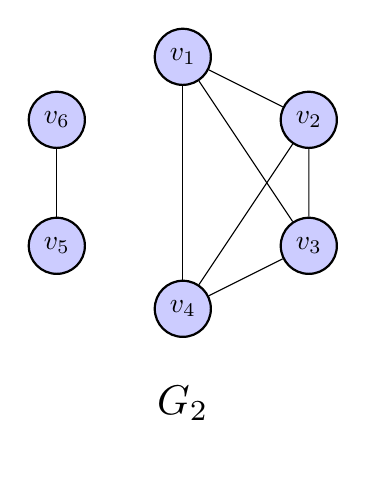
\begin{tikzpicture}
  [scale=.8,auto=left,every node/.style={circle,fill=blue!20,draw=black,thick}]
   \node (n1) at (2,4) {$v_1$};
  \node (n2) at (4,3)  {$v_2$};
  \node (n3) at (4,1)  {$v_3$};
  \node (n4) at (2,0) {$v_4$};
  \node (n5) at (0,1)  {$v_5$};
  \node (n6) at (0,3)  {$v_6$};

  \foreach \from/\to in {n1/n2,n2/n3,n1/n3, n1/n4, n2/n4, n3/n4,n5/n6}
    \draw (\from) -- (\to);

  % Etiqueta G_1 debajo del grafo
  \node[draw=none, fill=none, scale=1.5] at (2,-1.5) {$G_2$};

\end{tikzpicture}
}  \\[0.3cm]
    \resizebox{0.2\textwidth}{!}{\input{Preliminares_Grafos/Diagramas/Diag3.tex}} & 
    \hspace{1cm}
    \resizebox{0.2\textwidth}{!}{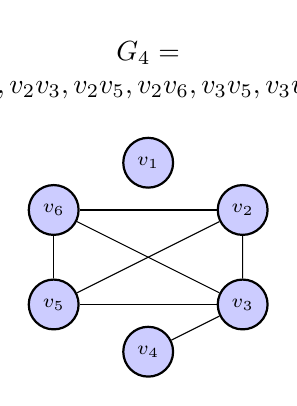
\begin{tikzpicture}
  [scale=.6, auto=left, 
   vertex/.style={circle, fill=blue!20, draw=black, thick, inner sep=2pt, minimum size=18pt}]

  \node[vertex] (n1) at (2,4) {$\scriptstyle v_1$};
  \node[vertex] (n2) at (4,3) {$\scriptstyle v_2$};
  \node[vertex] (n3) at (4,1) {$\scriptstyle v_3$};
  \node[vertex] (n4) at (2,0) {$\scriptstyle v_4$};
  \node[vertex] (n5) at (0,1) {$\scriptstyle v_5$};
  \node[vertex] (n6) at (0,3) {$\scriptstyle v_6$};

  \foreach \from/\to in {n3/n4,n2/n3, n2/n5, n2/n6, n3/n5, n3/n6, n5/n6}
    \draw (\from) -- (\to);

  \node[anchor=south, yshift=0.3cm] at (n1.north) {%
    \makebox[0pt][c]{%
      $\begin{array}{c}
        G_4=\\
        (V,\{v_3v_4, v_2v_3, v_2v_5, v_2v_6, v_3v_5, v_3v_6, v_5v_6\})
      \end{array}$%
    }%
  };
\end{tikzpicture}
} \\[0.3cm]
    \multicolumn{2}{c}{
      \resizebox{0.5\textwidth}{!}{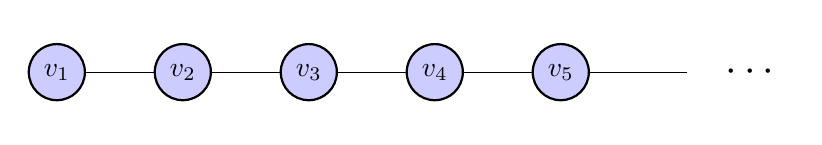
\begin{tikzpicture}
  [scale=.8,auto=left,every node/.style={circle,fill=blue!20,draw=black,thick}]
  \node (n1) at (0,0) {$v_1$};
  \node (n2) at (2,0)  {$v_2$};
  \node (n3) at (4,0)  {$v_3$};
  \node (n4) at (6,0) {$v_4$};
  \node (n5) at (8,0)  {$v_5$};

  \foreach \from/\to in {n1/n2,n2/n3, n3/n4, n4/n5}
    \draw (\from) -- (\to);

   %Flecha de (n5) a un nodo invisible en (10,0)   
   \draw (n5) -- (10,0);
   
   %Etiqueta de puntos suspensivos
   \node[draw=none, fill=none, scale=1.5] at (11,0) {$\cdots$};
   % Etiqueta G_1 debajo del grafo
%   \node[draw=none, fill=none, scale=1.5] at (6,-1.5) {$G_5$};
\end{tikzpicture}
}
    }
  \end{tabular}
  \caption{Grafos del Ejemplo \ref{Ejm:cuatro_grafos}}
  \label{fig:cuatro_grafos}
\end{figure}
La distribución particular de los puntos en el espacio, así como la forma en que las líneas son dibujadas es irrelevante; la única información que se importa es qué par de vértices están conectados mediante una arista y cuáles no. Solemos referirnos por \textit{grafo} también a la respectiva representación visual.\\
Notemos que la exigencia de que las aristas de un grafo sean $2-subconjuntos$ de vértices implica que si $uv\in A(G)$ entonces $u\neq v$, es decir, no hay aristas que unan un vértice con si mismo, lo que también expresamos diciendo que el grafo no tiene \textit{bucles}. Así mismo, entre dos vértices distintos $u,v\in V(G)$ podrá haber a lo más una arista, dependiendo de si $uv$ pertenece a $A(G)$ o no, es decir, se excluye la posibilidad de que hayan \textit{aristas paralelas} entre un par de vértices. En la literatura, se suele también hacer referencia a este tipo particular de grafos (no dirigidos, sin bucles y sin aristas paralelas) como \textit{grafos simples}. A lo largo del presente trabajo se entenderá \textit{grafo} y \textit{grafo simple} de manera indistinta.
\begin{Def}
   El \textbf{grado} de un grafo $G$, representado mediante $|G|$, es el cardinal del conjunto $V(G)$.
\end{Def}
Así por ejemplo, en el Ejemplo \ref{Ejm:cuatro_grafos}, el grado de los cuatro primeros grafos es $6$, mientras que $|G_5|=\aleph _0$. Los grafos pueden ser \textit{finitos, infinitos, contables}, etc. dependiendo del respectivo tamaño del conjunto $|G|$.
\begin{Def}
   En un grafo $G$ decimos que dos vértices $u,v\in V(G)$ son \textbf{adyacentes} si $uv\in A(G)$. Igualmente, decimos que el vértice $v\in V(G)$ es \textbf{incidente} con la arista $a\in A(G)$ si $v\in a$. 
\end{Def}
En el grafo $G_1$ del Ejemplo \ref{Ejm:cuatro_grafos}, los vértices $v_3$ y $v_4$ son adyacentes, los vértices $v_2$ y $v_5$ no son adyacentes, el vértice $v_6$ es incidente con la arista $v_1v_6$ y el vértice $v_4$ no es incidente con la arista $v_2v_3$.
